\documentclass[11pt]{charter}

% El títulos de la memoria, se usa en la carátula y se puede usar el cualquier lugar del documento con el comando \ttitle
\titulo{Adquisidor y display en tiempo real de datos de motores de combustión interna} 

% Nombre del posgrado, se usa en la carátula y se puede usar el cualquier lugar del documento con el comando \degreename
\posgrado{Carrera de Especialización en Sistemas Embebidos} 
%\posgrado{Carrera de Especialización en Internet de las Cosas} 
%\posgrado{Carrera de Especialización en Intelegencia Artificial}
%\posgrado{Maestría en Sistemas Embebidos} 
%\posgrado{Maestría en Internet de las cosas}

% Tu nombre, se puede usar el cualquier lugar del documento con el comando \authorname
\autor{Ing. Ignacio Moya}

% El nombre del director y co-director, se puede usar el cualquier lugar del documento con el comando \supname y \cosupname y \pertesupname y \pertecosupname
\director{Mg. Ing. Tomás Porreca}
\pertenenciaDirector{UNFLT} 
% FIXME:NO IMPLEMENTADO EL CODIRECTOR ni su pertenencia
\codirector{} % si queda vacio no se deberíá incluir 
\pertenenciaCoDirector{}

% Nombre del cliente, quien va a aprobar los resultados del proyecto, se puede usar con el comando \clientename y \empclientename
\cliente{Gastón Cabello}
\empresaCliente{Emprendimiento Personal}

% Nombre y pertenencia de los jurados, se pueden usar el cualquier lugar del documento con el comando \jurunoname, \jurdosname y \jurtresname y \perteunoname, \pertedosname y \pertetresname.
\juradoUno{Nombre y Apellido (1)}
\pertenenciaJurUno{pertenencia (1)} 
\juradoDos{Nombre y Apellido (2)}
\pertenenciaJurDos{pertenencia (2)}
\juradoTres{Nombre y Apellido (3)}
\pertenenciaJurTres{pertenencia (3)}
 
\fechaINICIO{23 de octubre de 2020}		%Fecha de inicio de la cursada de GdP \fechaInicioName
\fechaFINALPlanificacion{11 de diciembre de 2020} 	%Fecha de final de cursada de GdP
\fechaFINALTrabajo{22 de agosto de 2021}		%Fecha de defensa pública del trabajo final

\begin{document}

\maketitle
\thispagestyle{empty}
\pagebreak


\thispagestyle{empty}
{\setlength{\parskip}{0pt}
\tableofcontents{}
}
\pagebreak


\section{Registros de cambios}
\label{sec:registro}


\begin{table}[ht]
\label{tab:registro}
\centering
\begin{tabularx}{\linewidth}{@{}|c|X|c|@{}}
\hline
\rowcolor[HTML]{C0C0C0} 
Revisión & \multicolumn{1}{c|}{\cellcolor[HTML]{C0C0C0}Detalles de los cambios realizados} & Fecha      \\ \hline
1.0      & Creación del documento                                          & 23/10/2020 \\ \hline
1.1      & Avances en planificación del proyecto                           & 06/10/2020 \\ \hline
1.2      & Se agregaron las historias de usuario							 & 15/11/2020 \\ \hline
1.3      & Se completaron los puntos del 7 al 11							 & 23/11/2020 \\ \hline
%		   Con texto partido \newline
%		   En varias líneas \newline
%		   A propósito                                                     & dd/mm/aaaa \\ \hline
\end{tabularx}
\end{table}

\pagebreak



\section{Acta de constitución del proyecto}
\label{sec:acta}

\begin{flushright}
Buenos Aires, \fechaInicioName
\end{flushright}

\vspace{2cm}

Por medio de la presente se acuerda con el \authorname\hspace{1px} que su Trabajo Final de la \degreename\hspace{1px} se titulará ``\ttitle'', consistirá esencialmente en el prototipo preliminar de un sistema adquisidor de datos de motores de combustión interna con interfaz gráfica de usuario que será puesto a prueba sobre un motor de un vehículo Volskwagen Tipo 2, y tendrá un presupuesto preliminar estimado de 600 hs de trabajo y \textcolor{red}{\$XXX}, con fecha de inicio \fechaInicioName\hspace{1px} y fecha de presentación pública \fechaFinalName.

Se adjunta a esta acta la planificación inicial.

\vfill

% Esta parte se construye sola con la información que hayan cargado en el preámbulo del documento y no debe modificarla
\begin{table}[ht]
\centering
\begin{tabular}{ccc}
\begin{tabular}[c]{@{}c@{}}Ariel Lutenberg \\ Director posgrado FIUBA\end{tabular} & \hspace{2cm} & \begin{tabular}[c]{@{}c@{}}\clientename \\ \empclientename \end{tabular} \vspace{2.5cm} \\ 
\multicolumn{3}{c}{\begin{tabular}[c]{@{}c@{}} \supname \\ Director del Trabajo Final\end{tabular}} \vspace{2.5cm} \\
%\begin{tabular}[c]{@{}c@{}}\jurunoname \\ Jurado del Trabajo Final\end{tabular}     &  & \begin{tabular}[c]{@{}c@{}}\jurdosname\\ Jurado del Trabajo Final\end{tabular}  \vspace{2.5cm}  \\
%\multicolumn{3}{c}{\begin{tabular}[c]{@{}c@{}} \jurtresname\\ Jurado del Trabajo Final\end{tabular}} \vspace{.5cm}                                                                     
\end{tabular}
\end{table}

\section{Descripción técnica-conceptual del proyecto a realizar}
\label{sec:descripcion}

El sistema a desarrollar puede dividirse en dos partes, la adquisidora de datos y la interfaz gráfica. La primer parte consistirá de un circuito controlado por microprocesador montado cerca del motor del vehículo. El adquisidor tendrá la tarea de digitalizar las señales producidas por diversos sensores ubicados estratégicamente sobre el motor, para capturar las variables relacionadas con su funcionamiento. 

Luego, la información capturada por la parte adquisidora será transmitida a la segunda parte del sistema, la interfaz gráfica de usuario. La interfaz tendrá una pantalla para mostrar la información recibida, y entradas para que el usuario pueda tomar decisiones sobre la información que se muestra en pantalla. También tendrá una tarjeta SD o un dispositivo de memoria similar para poder guardar la información y ser descargada posteriormente. En la Figura \ref{fig:diagrama_de_bloques} el sistema está representado como diagrama en bloques con más detalle en los tipos de sensores a utilizar y la posible ubicación de las partes del sistema.

\vspace{25px}

\begin{figure}[htpb]
\centering 
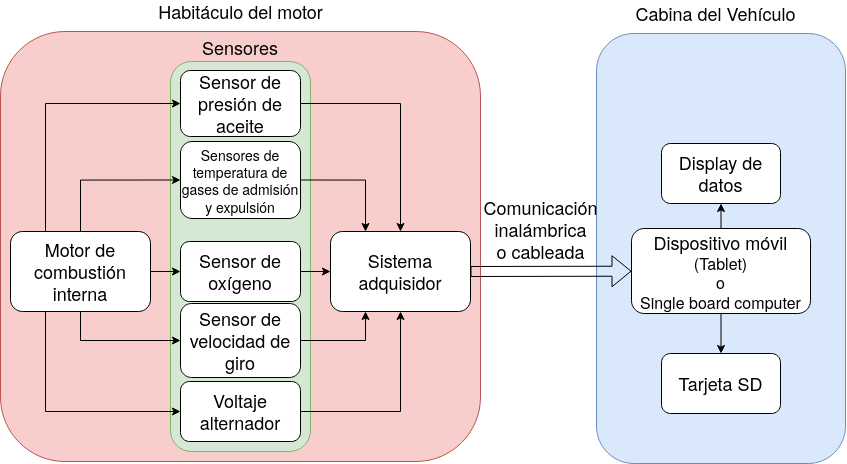
\includegraphics[width=.9\textwidth]{./Figuras/diagrama-proyecto.png}
\caption{Diagrama en bloques del sistema}
\label{fig:diagrama_de_bloques}
\end{figure}

\vspace{25px}

Lo que se quiere lograr con este sistema es que el usuario pueda ver en tiempo real en qué condiciones se encuentra funcionando el motor. Con esta información disponible se le otorga al usuario la capacidad de diagnosticar fallas antes de que le ocurran daños graves al motor. Se pretende ofrecer un gran aporte de valor a aquellas personas propietarias de vehículos antiguos que no tienen esta tecnología incorporada, dado que es muy costoso mantenerlos en funcionamiento óptimo, más que nada por la dificultad de conseguir repuestos. El sistema también tiene la posibilidad de aportar un gran valor en instituciones educativas técnicas que brinden enseñanza en la temática, brindando un contexto visual a fenómenos del funcionamiento de un motor que no podrían verse de otra forma.

Por esto es que se apunta a comercializar al sistema en forma de kit de sencilla instalación, apuntado a propietarios de automotores antiguos con intereses técnicos, mecánicos y también a instituciones educativas del rubro.

\section{Identificación y análisis de los interesados}
\label{sec:interesados}

\begin{table}[ht]
%\caption{Identificación de los interesados}
%\label{tab:interesados}
\begin{tabularx}{\linewidth}{@{}|l|X|X|l|@{}}
\hline
\rowcolor[HTML]{C0C0C0} 
Rol           & Nombre y Apellido & Organización 	& Puesto 	\\ \hline
%Auspiciante   & -                  						& -             	& -       	\\ \hline
Cliente       & \clientename      						&\empclientename	& -      	\\ \hline
%Impulsor      & -                 						& -            		& -       	\\ \hline
Responsable   & \authorname       						& LSE - FIUBA  		& Alumno 	\\ \hline
%Colaboradores & -                  						& -            		& -       	\\ \hline
Orientador    & \supname	      						& \pertesupname 	& Director \\ \hline
%Equipo        & -		         						& -            		& -      	\\ \hline
%Opositores    & -                  						& -            		& -        	\\ \hline
Usuario final & Propietarios de Vehículos antiguos, \newline  
				Mećanicos e Instituciones Educativas \newline  &            & \\ \hline
\end{tabularx}
\end{table}

\section{1. Propósito del proyecto}
\label{sec:proposito}

El propósito de este proyecto es el de desarrollar y construir un prototipo del sistema, instalarlo en una Volkswagen Tipo 2 modelo 1985 y analizar el funcionamiento de su motor en base a los datos visualizados.

\section{2. Alcance del proyecto}
\label{sec:alcance}

El alcance de este proyecto incluye:
\begin{itemize}
\item La elección de componentes electrónicos.
\item El diseño del circuito para amplificar las señales de los sensores.
\item El diseño del circuito impreso.
\item El desarrollo del firmware de la parte adquisidora.
\item El desarrollo del software de la interfaz gráfica de usuario.
\item La confección de un primer prototipo.
\item Los ensayos de verificación y validación con el prototipo.
\end{itemize}

El proyecto no incluye:
\begin{itemize}
\item La elección o desarrollo de un gabinete para la parte adquisidora.
\item El desarrollo de los componentes de montaje del sistema adquisidor.
\item El montaje del dispositivo para la interfaz gráfica en la cabina del vehículo.
\item La elección de sensores a utilizar.
\item Desarrollo del embalaje y documentación acompañante (e.g.: manual de usuario, prospecto).
\end{itemize}

\section{3. Supuestos del proyecto}
\label{sec:supuestos}

Para el desarrollo del presente proyecto se supone que:

\begin{itemize}
\item Los sensores ya fueron seleccionados, y que se cuenta con un sensor de oxígeno marca bosch y dos termocuplas para sensar la temperatura de los gases de admisión y escape, y también sensores para la temperatura y presión de aceite.
\item El resto de los materiales serán adquiridos por el Cliente.
\item Se cuenta con una placa EDU-CIAA sobre la cuál se desarrollará el firmware de la parte adquisidora.
\item Se cuenta con una tablet con pantalla táctil, puerto micro USB-OTG que corre sistema operativo Android.
\item Se supone que será fácil de conseguir las herramientas necesarias para el desarrollo y construcción del primer prototipo y su instalación en el vehículo. (e.g.: multímetro, osciloscopio, destornilladores, llaves, etc).
\end{itemize}

\section{4. Requerimientos}
\label{sec:requerimientos}

\begin{itemize}
\item Requerimientos generales del proyecto:
	\begin{itemize}
	\item \textbf{REQ-GEN-001:} Todo el código fuente del proyecto será almacenado bajo un sistema de control de versiones GIT.
	\item \textbf{REQ-GEN-002:} La documentación del código fuente del software embebido será llevada a cabo en los comentarios, siguiendo el formato de Doxygen.
	\item \textbf{REQ-GEN-003:} La documentación del software para la interfaz gráfica también será llevada a cabo en los comentarios. El formato será elegido por el responsable del proyecto.
	\end{itemize}
\item Requerimientos de la interfaz gráfica de usuario:
	\begin{itemize}
	\item \textbf{REQ-GUI-001:} La interfaz gráfica deberá poder mostrar figuras con la información de todos los sensores a la vez.
	\item \textbf{REQ-GUI-002:} El usuario tiene que poder elegir qué sensores ver al mismo tiempo y cuáles no desea ver.
	\item \textbf{REQ-GUI-003:} El usuario tiene que poder definir alarmas por valor máximo, para cada una de las variables.
	\item \textbf{REQ-GUI-004:} Las alarmas serán sonoras y visuales. El estilo de las alarmas será definido por el cliente durante el proceso de desarrollo de la interfaz gráfica.

	\end{itemize}
\item Requerimientos de la parte adquisidora:
	\begin{itemize}
	\item \textbf{REQ-ADQ-001:} El sistema tiene que adquirir la temperatura de los gases de admisión y escape, con un rango de temperatura entre 0"oC y 400"oC y una resolución menor igual a 0,5"oC Con una tasa de muestreo mayor igual a 1hz.
	\item \textbf{REQ-ADQ-002:} El sistema tiene que adquirir la temperatura del aceite del motor, con un rango de temperatura ente 0"oC y 400"oC y una resolución menor igual a 0,5"oC Con una tasa de muestreo mayor igual a 1hz.
	\item \textbf{REQ-ADQ-003:} El sistema tiene que adquirir la velocidad de giro del motor, en un rango entre 0 y 20.000 revoluciones por minuto, con una resolución menor igual a 500 r.p.m. Con una tasa de muestreo mayor igual a 5hz.
	\item \textbf{REQ-ADQ-004:} El sistema tiene que adquirir la proporción de oxígeno en los gases de escape llamada lambda, con un rango de 0 a 2 y una resolución menor igual a 0,1 lambda.
	\item \textbf{REQ-ADQ-005:} El sistema tiene que adquirir la presión de aceite del motor, con un rango de 0 a 100 psi y con una resolución menor igual a 1 psi.
	\item \textbf{REQ-ADQ-006:} El sistema debe comenzar a transmitir a la interfaz gráfica la información obtenida de los sensores en un tiempo no mayor a 1 segundo transcurrido el proceso de adquisición.
	
	\end{itemize}
\item Requerimientos de la comunicación entre las partes del sistema:
	\begin{itemize}
	\item \textbf{REQ-COMM-001:} Se permitirá que se pierda hasta 1 de cada 100 paquetes transmitidos.	
	\end{itemize}
\end{itemize}

\section{Historias de usuarios (\textit{Product backlog})}
\label{sec:backlog}

A continuación se detallan las historias de usuario, se asignó a cada historia un puntaje según que tan bien se puede entender el objetivo de la historia, su complejidad, su volumen y la incertidumbre de la tarea a realizar. Mientras mayor sea el puntaje quiere decir que será requerirá más trabajo para completar la historia. Los puntos se eligieron siguiendo la serie de Fibonacci, una historia solo puede como puntaje alguno de los siguientes números 1, 2, 3, 4, 5 y 13.

\begin{itemize}
\item \textbf{HU-001:} Como cliente quiero poder visualizar en una pantalla la información de los sensores en tiempo real en un mismo gráfico lineal para poder ver la evolución de las variables de los sensores.
	\begin{itemize}
	\item Ponderación: La complejidad de la historia complejidad es media y no es muy abarcativa, pero el responsable del proyecto tiene poca experiencia desarrollando interfaces gráficas. Se asignan 8 puntos de historia.
	\end{itemize}
\item \textbf{HU-002:} Como cliente quiero poder definir la escala del eje temporal del gráfico lineal, y elegir entre cinco valores distintos. (1, 10, 30, 60 y 120 minutos por división) para poder ver con con detalle fenómenos de corta y larga duración.
	\begin{itemize}
	\item Ponderación: La historia de usuario no debería abarcar mucho trabajo. Pero cómo en esta etapa todavía no se conoce como se implementarán los gráficos se le asignan 2 puntos de historia.
	\end{itemize}
\item \textbf{HU-003:} Como cliente quiero poder elegir qué sensores deben ser mostrados en pantalla y cuáles no, para poder darle prioridad a la información que es más relevante en ese momento.
	\begin{itemize}
	\item Ponderación: Se le asignan a esta historia de usuario 2 puntos de historia. Las razones son las mismas que para HU-002.
	\end{itemize}
\item \textbf{HU-004:} Como cliente quiero poder definir niveles para cada sensor individualmente, y que suene una alarma cuando algún valor supere dicho nivel para ser notificado al instante de que algo no funciona adecuadamente.
	\begin{itemize}
	\item Ponderación: Esta tarea es de complejidad media porque involucra reproducción de archivos de audio. Además en esta etapa todavía no esta completamente definido como será el sonido de la alarma. Se le asignan 8 puntos de historia.
	\end{itemize}
\item \textbf{HU-005:} Como cliente quiero poder descargar toda la información recolectada en una tarjeta SD o pendrive, para poder analizarla en otro momento.
	\begin{itemize}
	\item Ponderación: Volcar la información que está almacenada en la memoria no volátil del hardware de la interfaz gráfica a una tarjeta SD o pendrive no es una tarea muy compleja, aunque aún falta definir el tamaño y formato de la información a descargar. Se asignan 5 puntos de historia.
	\end{itemize}
\item \textbf{HU-006:} Como cliente quiero que el sistema comience a funcionar cuando se le da contacto al vehículo con la llave de ignición para poder ver en pantalla como funciona el motor durante el arranque.
	\begin{itemize}
	\item Ponderación: La historia de usuario es bastante compleja porque se deberá estudiar como funcionan los circuitos de ignición de un vehículo y diseñar un circuito que energice al sistema con el contacto de la llave. Se asignan 13 puntos de historia.
	\end{itemize}
\end{itemize}

\section{5. Entregables principales del proyecto}
\label{sec:entregables}

\begin{itemize}
\item Código fuente del firmware.
\item Código fuente del software de interfaz gráfica.
\item Documentación del firmware y software.
\item Esquemático del circuito.
\item Proyecto del circuito impreso.
\item Circuito impreso con componentes soldados en funcionamiento.
\item Memoria final.
\end{itemize}

\section{6. Desglose del trabajo en tareas}
\label{sec:wbs}

\begin{enumerate}
\item \textbf{Planificación.} (60 hs)
	\begin{enumerate}
	\item Plan de trabajo. (20 hs)
	\item Especificación de requerimientos de sistema. (20 hs)
	\item Definición de pruebas de verificación y validación. (20 hs)
	\end{enumerate}
\item \textbf{Diseño y construcción del hardware del equipo.} (65 hs)
	\begin{enumerate}
	\item Selección de componentes electrónicos. (10 hs)
	\item Diseño del esquemático del circuito. (20 hs)
	\item Diseño del circuito impreso. (20 hs)
	\item Diseño del esquema de interconexión. (5 hs)
	\item Montaje del prototipo. (10 hs)
	\end{enumerate}
\item \textbf{Diseño de la interfaz gráfica.} (165 hs)
	\begin{enumerate}
	\item Diseño de la arquitectura de software. (30 hs)
	\item Maquetación de la interfaz gráfica. (30 hs)
	\item Desarrollo del software. (30 hs)
	\item Pruebas de verificación. (30 hs)
	\item Modificaciones del software. (15 hs)
	\item Segunda ronda de pruebas de verificación. (30hs).
	\end{enumerate}
\item \textbf{Diseño e implementación del firmware} (170 hs).
	\begin{enumerate}
	\item Diseño de la arquitectura de software. (20 hs)
	\item Configuración con el entorno de desarrollo. (15 hs)
	\item Diseño del módulo adquisidor de temperaturas. (10hs)
	\item Diseño del módulo adquisidor de presión de aceite. (10 hs)
	\item Diseño del módulo adquisidor de relación de oxígeno. (10 hs)
	\item Diseño del módulo de transmisión de datos. (30 hs)
	\item Pruebas de verificación. (30hs)
	\item Modificaciones del software. (15hs)
	\item Segunda ronda de pruebas de verificación. (30hs).
	\end{enumerate}
\item \textbf{Etapa de validación.} (50 hs)
	\begin{enumerate}
	\item Pruebas de validación con el prototipo. (30hs)
	\item Ajustes luego de las pruebas de validación. (20hs)
	\end{enumerate}
\item \textbf{Cierre del proyecto.} (90 hs)
	\begin{enumerate}
	\item Informes de avance (20hs)
	\item Redacción de la memoria final (40hs)
	\item Correcciones a la memoria final (20hs)
	\item Presentación final (10hs).
	\end{enumerate}
\end{enumerate}

Cantidad total de horas: (600 hs)


\section{7. Diagrama de Activity On Node}
\label{sec:AoN}

En la figura \ref{fig:AoN} se detalla el desglose de tareas del proyecto como un diagrama "Activity on node", cada bloque representa una tarea y su color de fondo indica a que fase general del proyecto pertenece, la figura \ref{fig:leyenda-aon} describe este código de colores utilizado. El tiempo de las tareas está expresado en horas, se identifica un único camino crítico de duración de 360hs, el camino está sobresaltado con flechas de mayor grosor.

\begin{figure}[htpb]
\centering 
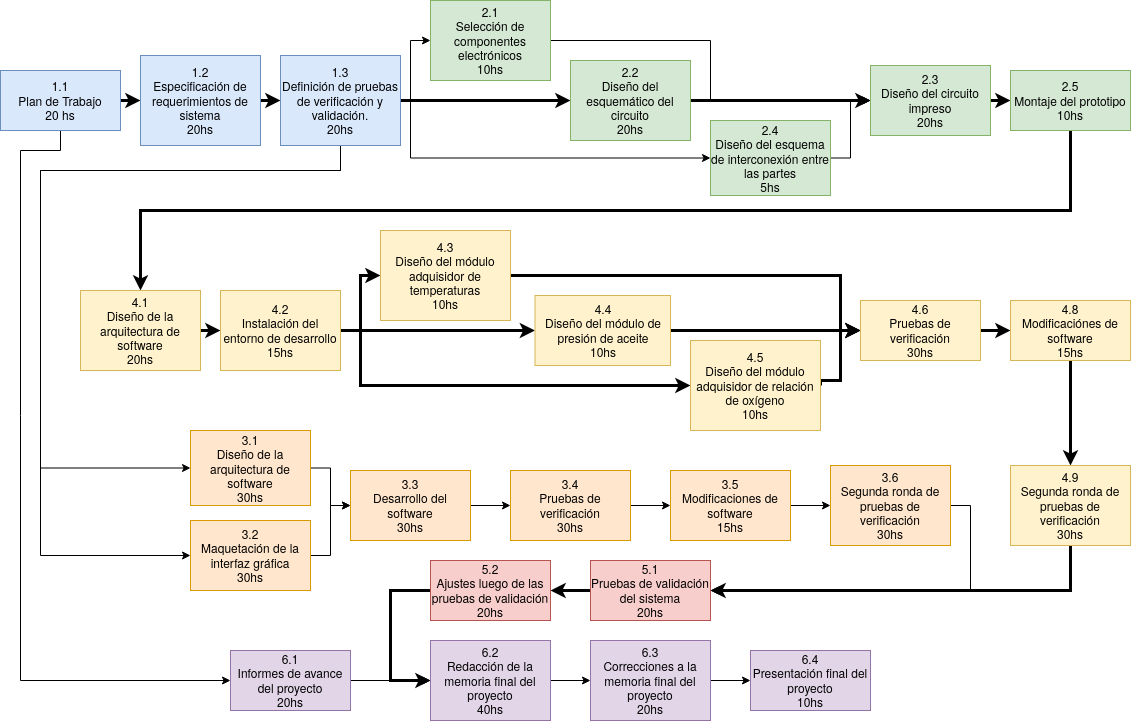
\includegraphics[angle=90, width=.9\textwidth]{./Figuras/activity-on-node.png}
\caption{Diagrama en \textit{Activity on Node}}
\label{fig:AoN}
\end{figure}

\begin{figure}[htpb]
\centering 
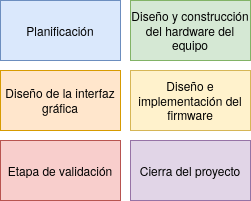
\includegraphics[width=.3\textwidth]{./Figuras/leyenda.png}
\caption{Código de colores del diagrama de la Figura\ref{fig:AoN}}
\label{fig:leyenda-aon}
\end{figure}


\section{8. Diagrama de Gantt}
\label{sec:gantt}

La figura \ref{fig:diagrama-gantt} es el diagrama de gantt para el proyecto y la figura \ref{fig:tabla-gantt} es una tabla con el detalle de todas las tareas de inicio con fecha de inicio, fecha de fin y duración de horas. De este diagrama se puede extraer que la fecha estimada de fin del proyecto es el 16 de Septiembre del 2021.

\begin{figure}[htpb]
\centering 
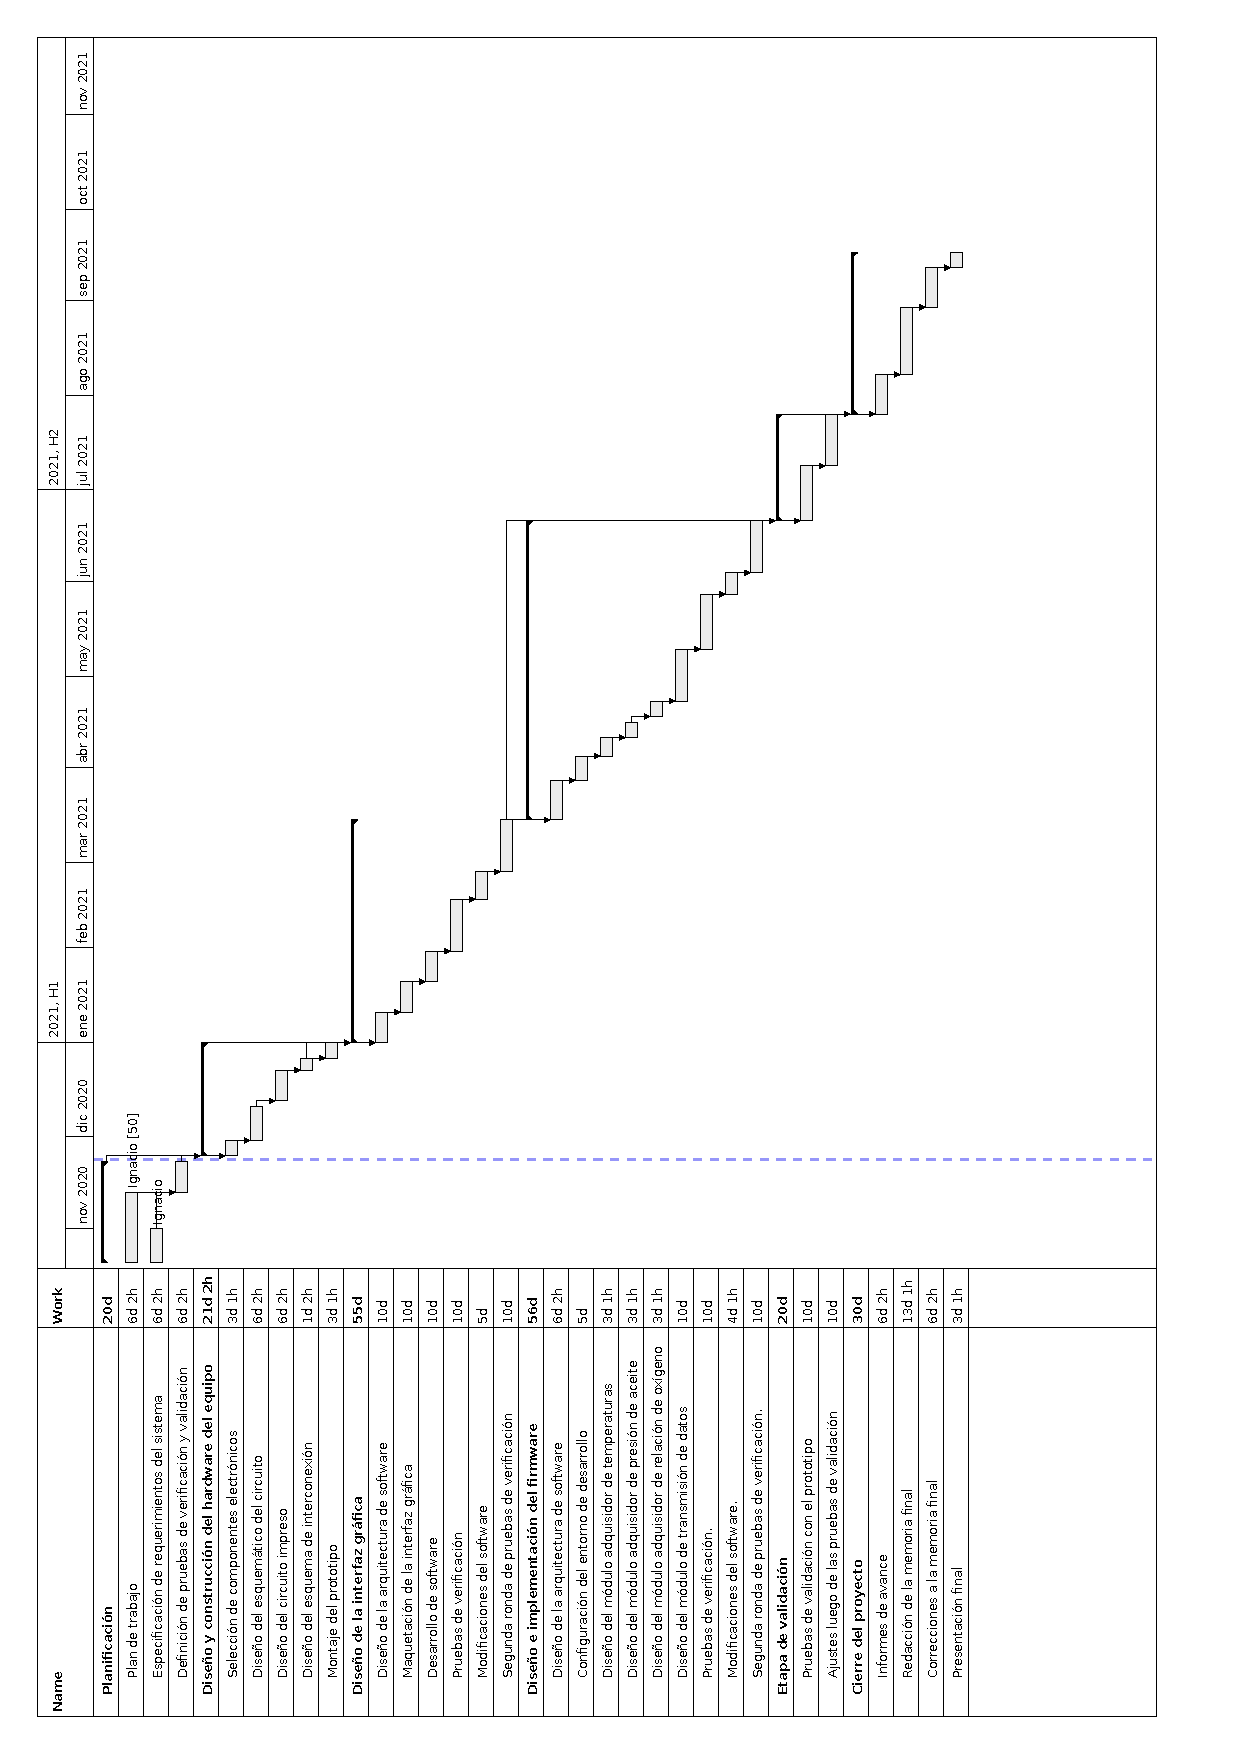
\includegraphics[width=1.05\textwidth]{./Figuras/diagrama-gantt.pdf}
\caption{Diagrama en \textit{Diagrama de gantt}}
\label{fig:diagrama-gantt}
\end{figure}

\begin{figure}[htpb]
\centering 
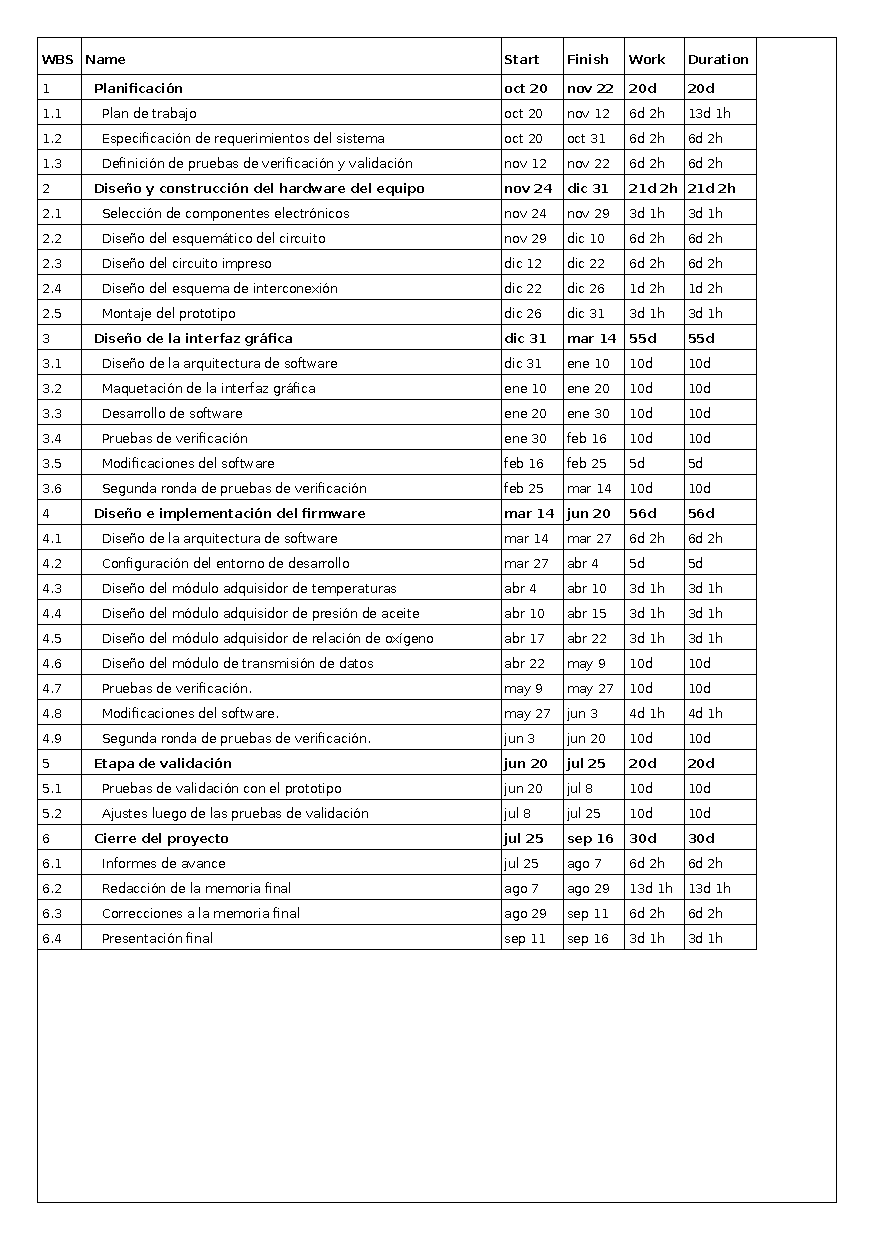
\includegraphics[width=.9\textwidth]{./Figuras/tabla-gantt.pdf}
\caption{Diagrama en \textit{Tabla de tareas con duración en horas y fecha de inicio}}
\label{fig:tabla-gantt}
\end{figure}




\section{9. Matriz de uso de recursos de materiales}
\label{sec:recursos}


\begin{table}
\label{tab:recursos}
\centering
\begin{tabularx}{\linewidth}{@{}|c|X|c|c|c|c|@{}}
\hline
\cellcolor[HTML]{C0C0C0} & \cellcolor[HTML]{C0C0C0} & \multicolumn{4}{c|}{\cellcolor[HTML]{C0C0C0}Recursos requeridos (horas)} \\ \cline{3-6} 
\multirow{-2}{*}{\cellcolor[HTML]{C0C0C0}\begin{tabular}[c]{@{}c@{}}Código\\ WBS\end{tabular}} &
\multirow{-2}{*}{\cellcolor[HTML]{C0C0C0}\begin{tabular}[c]{@{}c@{}}Nombre \\ tarea\end{tabular}} & PC & Soldador & Multímetro & Osciloscopio \\ \hline
 1.1 & Plan de Trabajo 											 & 20 &  &  &  \\ \hline
 1.2 & Especificación de requerimientos de software			 & 20 &  &  &  \\ \hline
 1.3 & Definición de pruebas de verificación y validación		 & 20 &  &  &  \\ \hline
 2.1 & Selección de componentes electrónicos					 & 10 &  &  &  \\ \hline
 2.2 & Diseño del esquemático del circuito						 & 20 &  &  &  \\ \hline
 2.3 & Diseño del circuito impreso								 & 20 &  &  &  \\ \hline
 2.4 & Diseño del esquema de interconexión						 & 5  &  &  &  \\ \hline
 2.5 & Montaje del prototipo										 &    & 8 & 1 & 1 \\ \hline 
 3.1 & Diseño de la arquitectura de software					 & 30 &  &  &  \\ \hline
 3.2 & Maquetación de la interfaz gráfica						 & 30 &  &  &  \\ \hline
 3.3 & Desarrollo del software									 & 30 &  &  &  \\ \hline
 3.4 & Pruebas de verificación									 & 30 &  &  &  \\ \hline
 3.5 & Modificaciones del software								 & 15 &  &  &  \\ \hline
 3.6 & Segunda ronda de pruebas de verificación				 & 30 &  &  &  \\ \hline
 4.1 & Diseño de la arquitectura de software					 & 20  &  &  &  \\ \hline
 4.2 & Configuración del entorno de desarrollo					 & 15  &  &  &  \\ \hline
 4.3 & Diseño del módulo adquisidor de temperaturas			 & 10 &  &  &  \\ \hline
 4.4 & Diseño del módulo adquisidor de presión de aceite		 & 10 &  &  &  \\ \hline
 4.5 & Diseño del módulo adquisidor de relación de oxígeno	 & 10 &  &  &  \\ \hline
 4.6 & Diseño del módulo de transmisión de datos				 & 30 &  &  &  \\ \hline
 4.7 & Pruebas de verificación									 & 20 &  & 5 & 5 \\ \hline
 4.8 & Modificaciones del software								 & 15 &  &  &  \\ \hline
 4.9 & Segunda ronda de pruebas de verificación				 & 30 &  &  &  \\ \hline
 5.1 & Pruebas de validación con el prototipo 					 & 20 & 2 & 4 & 4 \\ \hline 
 5.2 & Ajustes luego de las pruebas de verificación			 & 10  & 2 & 4 & 4 \\ \hline
 6.1 & Informes de avance											 & 20 &  &  &  \\ \hline
 6.2 & Redacción de la memoria final							 & 40 &  &  &  \\ \hline
 6.3 & Correcciones a la memoria final							 & 20 &  &  &  \\ \hline
 6.4 & Presentación final											 & 10 &  &  &  \\ \hline
\end{tabularx}
\end{table}

\section{10. Presupuesto detallado del proyecto}
\label{sec:presupuesto}

\begin{table}[htpb]
\centering
\begin{tabularx}{\linewidth}{@{}|X|c|r|r|@{}}
\hline
\rowcolor[HTML]{C0C0C0} 
\multicolumn{4}{|c|}{\cellcolor[HTML]{C0C0C0}COSTOS DIRECTOS} \\ \hline
\rowcolor[HTML]{C0C0C0} 
Descripción &
  \multicolumn{1}{c|}{\cellcolor[HTML]{C0C0C0}Cantidad} &
  \multicolumn{1}{c|}{\cellcolor[HTML]{C0C0C0}Valor unitario} &
  \multicolumn{1}{c|}{\cellcolor[HTML]{C0C0C0}Valor total} \\ \hline
 Mano de obra &
  \multicolumn{1}{c|}{600} &
  \multicolumn{1}{c|}{750} &
  \multicolumn{1}{c|}{450.000} \\ \hline
 EDU-CIAA&
  \multicolumn{1}{c|}{1} &
  \multicolumn{1}{c|}{6.000} &
  \multicolumn{1}{c|}{6.000} \\ \hline
 Componentes electrónicos&
  \multicolumn{1}{c|}{1} &
  \multicolumn{1}{c|}{10.000} &
  \multicolumn{1}{c|}{10.000} \\ \hline
 Fabricación PCB&
  \multicolumn{1}{c|}{1} &
  \multicolumn{1}{c|}{12.000} &
  \multicolumn{1}{c|}{12.000} \\ \hline
 Consumibles&
  \multicolumn{1}{c|}{1} &
  \multicolumn{1}{c|}{3.000} &
  \multicolumn{1}{c|}{3.000} \\ \hline
\multicolumn{3}{|c|}{SUBTOTAL} &
  \multicolumn{1}{c|}{481.000} \\ \hline
\rowcolor[HTML]{C0C0C0} 
\multicolumn{4}{|c|}{\cellcolor[HTML]{C0C0C0}COSTOS INDIRECTOS} \\ \hline
\rowcolor[HTML]{C0C0C0} 
Descripción &
  \multicolumn{1}{c|}{\cellcolor[HTML]{C0C0C0}Cantidad} &
  \multicolumn{1}{c|}{\cellcolor[HTML]{C0C0C0}Valor unitario} &
  \multicolumn{1}{c|}{\cellcolor[HTML]{C0C0C0}Valor total} \\ \hline
30\% de los costos directos  &
	\multicolumn{1}{c|}{1} &
	\multicolumn{1}{c|}{144.300} &
	\multicolumn{1}{c|}{144.300}
   \\ \hline
\multicolumn{3}{|c|}{SUBTOTAL} &
  \multicolumn{1}{c|}{144.300} \\ \hline
\rowcolor[HTML]{C0C0C0}
\multicolumn{3}{|c|}{TOTAL} &
\multicolumn{1}{c|}{625.300}
   \\ \hline
\end{tabularx}%
\end{table}


\section{11. Matriz de asignación de responsabilidades}
\label{sec:responsabilidades}
\begin{table}[htpb]
\centering
\resizebox{\textwidth}{!}{%
%\begin{tabular}{|c|c|c|c|c|c|}
\begin{tabular}{@{}|c|c|c|c|c|@{}}
\hline
\rowcolor[HTML]{C0C0C0} 
\cellcolor[HTML]{C0C0C0} &
  \cellcolor[HTML]{C0C0C0} &
  \multicolumn{3}{c|}{\cellcolor[HTML]{C0C0C0}Listar todos los nombres y roles del proyecto} \\ \cline{3-5} 
\rowcolor[HTML]{C0C0C0} 
\cellcolor[HTML]{C0C0C0} &
  \cellcolor[HTML]{C0C0C0} &
  Responsable &
  Orientador &
  Cliente \\ \cline{3-5} 
\rowcolor[HTML]{C0C0C0} 
\multirow{-3}{*}{\cellcolor[HTML]{C0C0C0}\begin{tabular}[c]{@{}c@{}}Código\\ WBS\end{tabular}} &
  \multirow{-3}{*}{\cellcolor[HTML]{C0C0C0}Nombre de la tarea} &
  \authorname &
  \supname &
  \clientename\\ \hline
 %Responsable Orientador Equipo Cliente
 1.1 & Plan de trabajo											 & P  & C   & A  \\ \hline
 1.2 & Especificación de requisitos del sistema				 & P  & C   & A  \\ \hline
 1.3 & Definición de pruebas de verificación y validación		 & P  & C   & A  \\ \hline
 2.1 & Selección de componentes electrónicos					 & P  & C/A &  \\ \hline
 2.2 & Diseño del esquemático del circuito						 & P  & C/A &  \\ \hline
 2.3 & Diseño del circuito impreso								 & P  & C/A &  \\ \hline
 2.4 & Diseño del esquema de interconexión						 & P  & C/A &  \\ \hline
 2.5 & Montaje del prototipo									 	 & P  & C/A &  \\ \hline
 3.1 & Diseño de la arquitectura de software					 & P  & C/A &  \\ \hline
 3.2 & Maquetación de la interfaz gráfica   					 & P  & C   & A  \\ \hline
 3.3 & Desarrollo de software									 & P  & C/A &  \\ \hline
 3.4 & Pruebas de verificación									 & P  & C/A & I  \\ \hline
 3.5 & Modificaciones de software								 & P  & C/A &  \\ \hline
 3.6 & Segunda ronda de pruebas de verificación				 & P  & C/A & I  \\ \hline
 4.1 & Diseño de la arquitectura de software					 & P  & C/A &  \\ \hline
 4.2 & Configuración del entorno de desarrollo					 & P  & C/A &  \\ \hline
 4.3 & Diseño del módulo adquisidor de temperaturas			 & P  & C/A &  \\ \hline
 4.4 & Diseño del módulo de presión de aceite					 & P  & C/A &  \\ \hline
 4.5 & Diseño del módulo adquisidor de relación de oxígeno		 & P  & C/A &  \\ \hline
 4.6 & Diseño del módulo de comunicación						 & P  & C/A &  \\ \hline
 4.7 & Pruebas de verificación									 & P  & C/A & I  \\ \hline
 4.8 & Modificaciones de software								 & P  & C/A &  \\ \hline
 4.9 & Segunda ronda de pruebas de verificación				 & P  & C/A & I  \\ \hline
 5.1 & Pruebas de validación del sistema			             & P  & C & A \\ \hline
 5.2 & Ajustes luego de las pruebas de validación				 & P  & C & A \\ \hline
 6.1 & Informes de avance  										 & P  & A & I  \\ \hline
 6.2 & Redacción de la memoria final				 			 & P  & A & I \\ \hline
 6.3 & Correcciones a la memoria final 							 & P  & A & I  \\ \hline
 6.4 & Presentación final  										 & P  & A & I  \\ \hline
\end{tabular}%
}
\end{table}

\section{12. Gestión de riesgos}
\label{sec:riesgos}

Riesgo 1: Incumplimiento de la fecha de cierre de proyecto producto de una planificación errónea.
\begin{itemize}
\item Severidad (9): El incumplimiento de la fecha pactada no sólo afecta a la fecha de cierre sino que también afecta al presupuesto del proyecto por las horas de trabajo extra que no estuvieron contadas en la planificación inicial.
\item Probabilidad de ocurrencia (4): El responsable del proyecto tiene poca experiencia en interfaces gráficas. Es posible que las horas destinadas a esas tareas estén subestimadas.
\end{itemize}  

Riesgo 2: Dificultad para conseguir componentes y materiales.
\begin{itemize}
\item Severidad (7): No poder conseguir materiales y/o componentes implica demoras y un aumento del costo del proyecto. Se ser imposible de conseguir un componente o parte se tendría que rediseñar para acomodar el nuevo componente o parte. 
\item Ocurrencia (8): En Argentina es difícil de conseguir partes o materiales fabricadas en el extranjero debido a las restricciones e impuestos a las importaciones. Esto hace que el riesgo tenga alta ocurrencia.
\end{itemize}

Riesgo 3: Incumplimiento de los requisitos del proyecto.
\begin{itemize}
\item Severidad (10): Un incumplimiento con los requisitos del proyecto significa que el proyecto no pudo ser completado.
\item Ocurrencia (2): Es posible que los requisitos sean muy ambiciosos para la tecnología disponible y que no puedan alcanzarse, aunque en un primer análisis esto no parece que sea muy probable.
\end{itemize}

Riesgo 4: Pérdida de componentes electrónicos durante ensayos con hardware involucrado.
\begin{itemize}
\item Severidad (6): La pérdida de materiales implica demoras y costos agregados ya que habría que volver a comprar el material perdido y volver a esperar a que llegue en caso de que sean comprados por un proveedor que no es local.
\item Ocurrencia (2): Puede suceder que durante alguno de los ensayos algún componente quede inutilizable producto de alguna conexión errónea o error humano, sin embargo el responsable del proyecto es ingeniero electrónico y tiene experiencia trabajando con hardware.
\end{itemize}

Riesgo 5: Pérdida de documentos y/o archivos del desarrollo.
\begin{itemize}
\item Severidad (10): La pérdida de documentación o archivos ligados al desarrollo implicaría tener que rehacer todo el trabajo realizado hasta ese punto. Las demoras agregadas implicarían no cumplir con la fecha de cierre del proyecto.
\item Ocurrencia (3): Toda la información sobre el proyecto estará guardada digitalmente en una computadora personal. Es posible que se pierda información a causa de una falla del disco rígido o que el responsable del proyecto olvide de guardar los cambios generados.
\end{itemize}

\begin{table}[htpb]
\centering
\begin{tabularx}{\linewidth}{@{}|X|X|X|X|X|X|X|@{}}
\hline
\rowcolor[HTML]{C0C0C0} 
Riesgo	& S		& O	& RPN	& S*		& O* & RPN* \\ \hline
1 		& 9		& 4	&  36	& 9		& 2  & 18	\\ \hline
2		& 7		& 8	&  56	& 7		& 2  & 14	\\ \hline
3		& 10		& 2	&  20	& -		& -  & -		\\ \hline
4		& 6		& 2	&  12	& -		& -  & -		\\ \hline
5		& 10		& 3	&  30	& 10		& 1  & 10	\\ \hline
\end{tabularx}%
\end{table}

Se tomarán medidas de mitigación en los riesgos cuyos números de RPN sean mayores o igual a 30.

Riesgo 1: Incumplimiento de la fecha de cierre de proyecto producto de una planificación errónea.
\begin{itemize}
\item Plan de mitigación: Se sobreestimaron las horas relacionadas con el desarrollo de la interfaz gráfica por un factor de un 30\%.
\item Severidad(9).
\item Ocurrencia(2).
\end{itemize}  

Riesgo 2: Dificultad para conseguir componentes y materiales.
\begin{itemize}
\item Plan de mitigación: En el diseño de hardware sólo se utilizaran componentes que se consigan de proveedores que estén en Argentina. Minimizando la cantidad de componentes a importar lo máximo posible.
\item Severidad(7)
\item Ocurrencia(2)
\end{itemize}

Riesgo 5: Pérdida de documentos y/o archivos del desarrollo.
\begin{itemize}
\item Plan de mitigación: Cada archivo del proyecto tendrá un espejo guardado en la nube. Todo el software será alojado en repositorios git en github. El resto de los archivos serán guardados dentro del Google Drive del responsable del proyecto y serán compartidos con el cliente y con el director.
\item Severidad(10)
\item Ocurrencia(1)
\end{itemize}

\section{13. Gestión de la calidad}
\label{sec:calidad}

\begin{itemize} 
\item Req \#1: REQ-GEN-001: Todo el código fuente del proyecto será almacenado bajo un
sistema de control de versiones GIT.
Verificación y validación:
\begin{itemize}
\item Verificación: Previo al comienzo de la etapa de desarrollo de software se confeccionará una lista con los proyectos tendrán que estar bajo control de versiones y la dirección URL al repositorio remoto de cada proyecto. En cada etapa se verificará que esa lista esté completa.
\item Validación: Se compartirá al cliente la lista con los enlaces a los repositorios de todos los códigos fuente.
\end{itemize}
\end{itemize}

\begin{itemize} 
\item Req \#2: REQ-GEN-002: La documentación del código fuente del software embebido será
llevada a cabo en los comentarios, siguiendo el formato de Doxygen.
Verificación y validación:
\begin{itemize}
\item Verificación: Se verificará que todas las funciones tengan su documentación asociada en el código fuente y que se genere de forma correcta en el resultado de Doxygen.
\item Validación: Se validará con la aprobación del cliente sobre la documentación entregada.
\end{itemize}
\end{itemize}

\begin{itemize} 
\item Req \#3: REQ-GEN-003: La documentación del software para la interfaz gráfica también
será llevada a cabo en los comentarios. El formato será elegido por el responsable del
proyecto.
Verificación y validación:
\begin{itemize}
\item Verificación: Se verificará que todas las funciones tengan su documentación asociada en el código fuente.
\item Validación: Se validará con la aprobación del cliente sobre la documentación entregada.
\end{itemize}
\end{itemize}

\begin{itemize} 
\item Req \#4: REQ-GUI-001: La interfaz gráfica deberá poder mostrar figuras con la información
de todos los sensores a la vez.
Verificación y validación:
\begin{itemize}
\item Verificación: Se verificará visualmente.
\item Validación: El cliente validará este requisito en la demostración del equipo.
\end{itemize}
\end{itemize}

\begin{itemize} 
\item Req \#5: REQ-GUI-002: El usuario tiene que poder elegir qué sensores ver al mismo tiempo
y cuáles no desea ver.
Verificación y validación:
\begin{itemize}
\item Verificación: Se verificará visualmente y con pruebas unitarias.
\item Validación: El cliente validará este requisito en la demostración del equipo.
\end{itemize}
\end{itemize}

\begin{itemize} 
\item Req \#6: REQ-GUI-003: El usuario tiene que poder definir alarmas por valor máximo, para
cada una de las variables.
Verificación y validación:
\begin{itemize}
\item Verificación: Se verificará mediante pruebas unitarias.
\item Validación: El cliente validará este requisito en la demostración del equipo.
\end{itemize}
\end{itemize}

\begin{itemize} 
\item Req \#7: REQ-GUI-004: Las alarmas serán sonoras y visuales. El estilo de las alarmas será
definido por el cliente durante el proceso de desarrollo de la interfaz gráfica.
Verificación y validación:
\begin{itemize}
\item Verificación: Se simularán varias situaciones de alarma con un firmware especial de la parte adquisidora para comprobar que la alarma se active correctamente.
\item Validación: En la demostración del equipo se extraerán los sensores del motor y se forzará una situación de alarma físicamente (e.g.: Sosteniendo una termocupla sobre la llama de un encendedor).
\end{itemize}
\end{itemize}

\begin{itemize} 
\item Req \#8: REQ-ADQ-001: El sistema tiene que adquirir la temperatura de los gases de
admisión y escape, con un rango de temperatura entre 0. o C y 400. o C y una resolución
menor igual a 0,5. o C Con una tasa de muestreo mayor igual a 1hz.
Verificación y validación:
\begin{itemize}
\item Verificación: Se verificará contrastando los resultados de la medición con los resultados de otro termómetro que se utilizará como patrón.
\item Validación: Se entregarán los resultados del ensayo al cliente.
\end{itemize}
\end{itemize}

\begin{itemize} 
\item Req \#9: REQ-ADQ-002: El sistema tiene que adquirir la temperatura del aceite del motor,
con un rango de temperatura ente 0. o C y 400. o C y una resolución menor igual a
0,5. o C Con una tasa de muestreo mayor igual a 1hz.
Verificación y validación:
\begin{itemize}
\item Verificación: Se verificará contrastando los resultados de la medición con los resultados de otro termómetro que se utilizará como patrón.
\item Validación: Se entregarán los resultados del ensayo al cliente.
\end{itemize}
\end{itemize}

\begin{itemize} 
\item Req \#10: REQ-ADQ-003: El sistema tiene que adquirir la velocidad de giro del motor, en
un rango entre 0 y 20.000 revoluciones por minuto, con una resolución menor igual
a 500 r.p.m. Con una tasa de muestreo mayor igual a 5hz.
Verificación y validación:
\begin{itemize}
\item Verificación: Se simulará el sensor de velocidad de giro con otro pin GPIO de la misma placa.
\item Validación: Se contrastará los resultados del equipo con los resultado del tacómetro del motor.
\end{itemize}
\end{itemize}

\begin{itemize} 
\item Req \#11: REQ-ADQ-004: El sistema tiene que adquirir la proporción de oxígeno en los gases
de escape llamada lambda, con un rango de 0 a 2 y una resolución menor igual a 0,1
lambda.
Verificación y validación:
\begin{itemize}
\item Verificación: Se simulará la señal del sensor lambda con una fuente de tensión variable.
\item Validación: Se contrastarán los resultado del equipo con los de otro sensor de oxígeno.
\end{itemize}
\end{itemize}

\begin{itemize} 
\item Req \#12: REQ-ADQ-005: El sistema tiene que adquirir la presión de aceite del motor, con
un rango de 0 a 100 psi y con una resolución menor igual a 1 psi.
Verificación y validación:
\begin{itemize}
\item Verificación: Se simulará la señal del sensor de presión con una fuente de tensión variable.
\item Validación: Se contrastará los resultados del equipo con los resultados de otro sensor de presión.
\end{itemize}
\end{itemize}

\begin{itemize} 
\item Req \#13: REQ-ADQ-006: El sistema debe comenzar a transmitir a la interfaz gráfica la
información obtenida de los sensores en un tiempo no mayor a 1 segundo transcurrido
el proceso de adquisición.
Verificación y validación:
\begin{itemize}
\item Verificación: Se realizarán ensayos para medir el tiempo de encendido de la parte adquisidora utilizando el debugger integrado y un firmware especial para reportar el tiempo hasta la transmisión del primer paquete.
\item Validación: Se entregarán al cliente los resultados de esos ensayos.
\end{itemize}
\end{itemize}

\begin{itemize} 
\item Req \#14: REQ-COMM-001: Se permitirá que se pierda hasta 1 de cada 100 paquetes
transmitidos.
Verificación y validación:
\begin{itemize}
\item Verificación: En el software se incluirá un modo de "desarrollo" en el que cada parte reportará la cantidad de paquetes enviados/recibidos. Se calculará la cantidad de paquetes perdidos cada cien enviados a partir de un total de 10.000 paquetes enviados.
\item Validación: Se entregarán al cliente los resultados de esos ensayos.
\end{itemize}
\end{itemize}

\section{14. Comunicación del proyecto}
\label{sec:comunicaciones}

El plan de comunicación del proyecto es el siguiente:

\begin{table}[htpb]
\centering
\begin{tabularx}{\linewidth}{@{}|X|C{2.4cm}|C{3cm}|C{1.8cm}|C{2cm}|C{2.1cm}|@{}}
\hline
\rowcolor[HTML]{C0C0C0} 
\multicolumn{6}{|c|}{\cellcolor[HTML]{C0C0C0}PLAN DE COMUNICACIÓN DEL PROYECTO}           \\ \hline
\rowcolor[HTML]{C0C0C0} 
¿Qué comunicar?					& Audiencia			& Propósito					& Frecuencia & Método de comunicac. & Responsable \\ \hline
Definicón de objetivos y alcances& Director y cliente	& Evaluación de factibilidad & Al inicio del proyecto & Correo electrónico & \authorname \\ \hline
Informe de avances				& Cliente, director y jurado & Comunicar el trabajo realizado y los problemas resueltos  & A la mitad del proyecto & Correo electrónico o video-llamada	& \authorname \\ \hline
Resolución de problemas			& Director          & Agilizar la resolución de problemas & Cuando sea necesario & Correo electrónico o video-llamada & \authorname	\\ \hline
Finalización y cierre			& Director, jurado y cliente &  & En la última etapa del proyecto & Correo electrónico y video-llamada & \authorname\\ \hline
\end{tabularx}
\end{table}

\section{15. Gestión de compras}
\label{sec:compras}

	Para este proyecto se prevé la compra de componentes electrónicos y la fabricación de un circuito impreso. Sólo se utilizarán proveedores que se encuentren en Argentina, de ser imposible conseguir algún componente en el mercado local se intentará conseguirlo de algún proveedor internacional como puede ser Digikey, Mouser o Arrow.
	La fabricación del circuito impreso se encargará con alguno de los fabricantes que se encuentran en la ciudad de Rosario para disminuir los tiempos de envío. En Rosario hay dos fabricantes de circuitos impresos, LAM Circuitos Impresos y ADN Electrónica.

\section{16. Seguimiento y control}
\label{sec:seguimiento}

\begin{longtable}{|m{1cm}|m{3.5cm}|m{2.2cm}|m{2cm}|m{3cm}|m{1.5cm}|}
%\hline
%\rowcolor[HTML]{C0C0C0} 
%\multicolumn{6}{|c|}{\cellcolor[HTML]{C0C0C0}SEGUIMIENTO DE AVANCE}                                                                       \\ \hline
%\rowcolor[HTML]{C0C0C0} 
%Tarea del WBS 			& Indicador de avance & Frecuencia de reporte & Resp. de seguimiento & Persona a ser informada & Método de comunic. \\ \hline
%\endfirsthead

%1. Planificación									& Plan de trabajo y especificación de requisitos de software & Al finalizar la tarea & \authorname & %\clientename, \supname & correo electrónico \\ \hline
%2. Diseño y construcción del hardware del equipo	& Documento de especificación de requisitos de software  & Al finalizar la tarea & \authorname & \clientename, \supname & correo electrónico \\ \hline
%3. Diseño de la interfaz gráfica					&  &  & \authorname & \clientename, \supname & correo electrónico \\ \hline
%4. Diseño e implementación del firmware			&  &  & \authorname & \clientename, \supname & correo electrónico \\ \hline
%5. Etapa de validación							&  &  & \authorname & \clientename, \supname & correo electrónico \\ \hline
%6. Cierre del proyecto							&  &  & \authorname & \clientename, \supname & correo electrónico \\ \hline

\hline
\rowcolor[HTML]{C0C0C0} 
\multicolumn{6}{c}{\cellcolor[HTML]{C0C0C0}SEGUIMIENTO DE AVANCE}                                                                       \\ \hline
\rowcolor[HTML]{C0C0C0} 
Tarea del WBS 			& Indicador de avance & Frecuencia de reporte & Resp. de seguimiento & Persona a ser informada & Método de comunic. \\ \hline
\endhead

\multicolumn{6}{c}{Continúa}
\endfoot

\endlastfoot
1.1 & Documento del plan de trabajo& Al finalizar la tarea & \authorname & \clientename, \supname & correo electrónico \\ \hline
1.2 & Documento de especificación de requisitos de software & Al finalizar la tarea & \authorname & \clientename, \supname & correo electrónico \\ \hline
1.3 & Documento de especificación de requisitos de testing & Al finalizar la tarea & \authorname & \clientename, \supname & correo electrónico \\ \hline
2.1 a 2.5 & Entregable de cada tarea entregado & Cada 15 días y al finalizar cada tarea & \authorname & \clientename, \supname & correo electrónico \\ \hline
3.1 a 3.6 & Cantidad de módulos resueltos y resultados de pruebas unitarias & Cada 15 días y al finalizar cada tarea & \authorname & \supname & correo electrónico \\ \hline
4.1 a 4.9 & Cantidad de módulos resueltos y resultados de pruebas unitarias & Cada 15 días y al finalizar cada subtarea & \authorname & \supname & correo electrónico \\ \hline
5 a 5.2 & Cantidad de pruebas de validación exitosas & Semanalmente y al finalizar & \authorname & \clientename, \supname & correo electrónico \\ \hline
6.1 a 6.4 & Memoria final del proyecto y cantidad de entregables entregados & Al finalizar & \authorname & \clientename, \supname & correo electrónico \\ \hline

%1. Planificación
%2. Diseño y construcción del hardware
%3. Diseño GUI
%4. Firmw
%5. Validación
%6. Cierre

\end{longtable}

\section{17. Procesos de cierre}    
\label{sec:cierre}

Pautas de trabajo que se seguirán para analizar si se respetó el Plan de Proyecto original:
\begin{itemize}
\item Responsable: \authorname
\item Procedimiento: Se realizará una reunión de cierre del proyecto para evaluar el cumplimiento del plan de proyecto origina, de la reunión participaran \clientename, \supname y el \authorname
\item Pauta: La evaluación se realizará según si todos los requisitos fueron cumplidos en tiempo y costo estimados.
\end{itemize}
Identificación de las técnicas y procedimientos útiles e inútiles que se utilizaron, y los problemas que surgieron y cómo se solucionaron:
\begin{itemize}
\item Responsable: \authorname
\item Procedimiento: En análisis será presentado en forma oral y escrita en la memoria final y en la presentación del proyecto.
\end{itemize}
Indicar quién organizará el acto de agradecimiento a todos los interesados, y en especial al equipo de trabajo y colaboradores:
\begin{itemize}
\item Responsable: \authorname
\item Procedimiento: Al finalizar la presentación del proyecto ante el jurado se agradecerá a todos los involucrados en el proyecto incluyendo a los colaboradores.
\end{itemize}

\end{document}
